\chapter{Principal Component Analysis}
\label{chap:pca}
The Principal Component Analysis (\gls{pca}) is an unsupervised machine learning technique which is often used to reduce the dimensionality of a given feature set.
A data set is decorrelated by diagonalization of the respective covariance matrix and subsequently ordered by the standard deviation of each feature.
A reduction is achieved by pruning features with a low standard deviation (after being decorrelated).

The latter step is driven by the motivation that features with low standard deviations carry less information than is needed to describe the distribution of the data.
We note, however, that in classification tasks the information needed to distinguish between a given set of categories can be dominantly encoded in the features with a low standard deviation.
We show such an example in Fig.~\ref{fig:apdx_pca}.
\begin{figure}[htbp]
    \centering
    \begin{subfigure}{.49\textwidth}
        \centering
        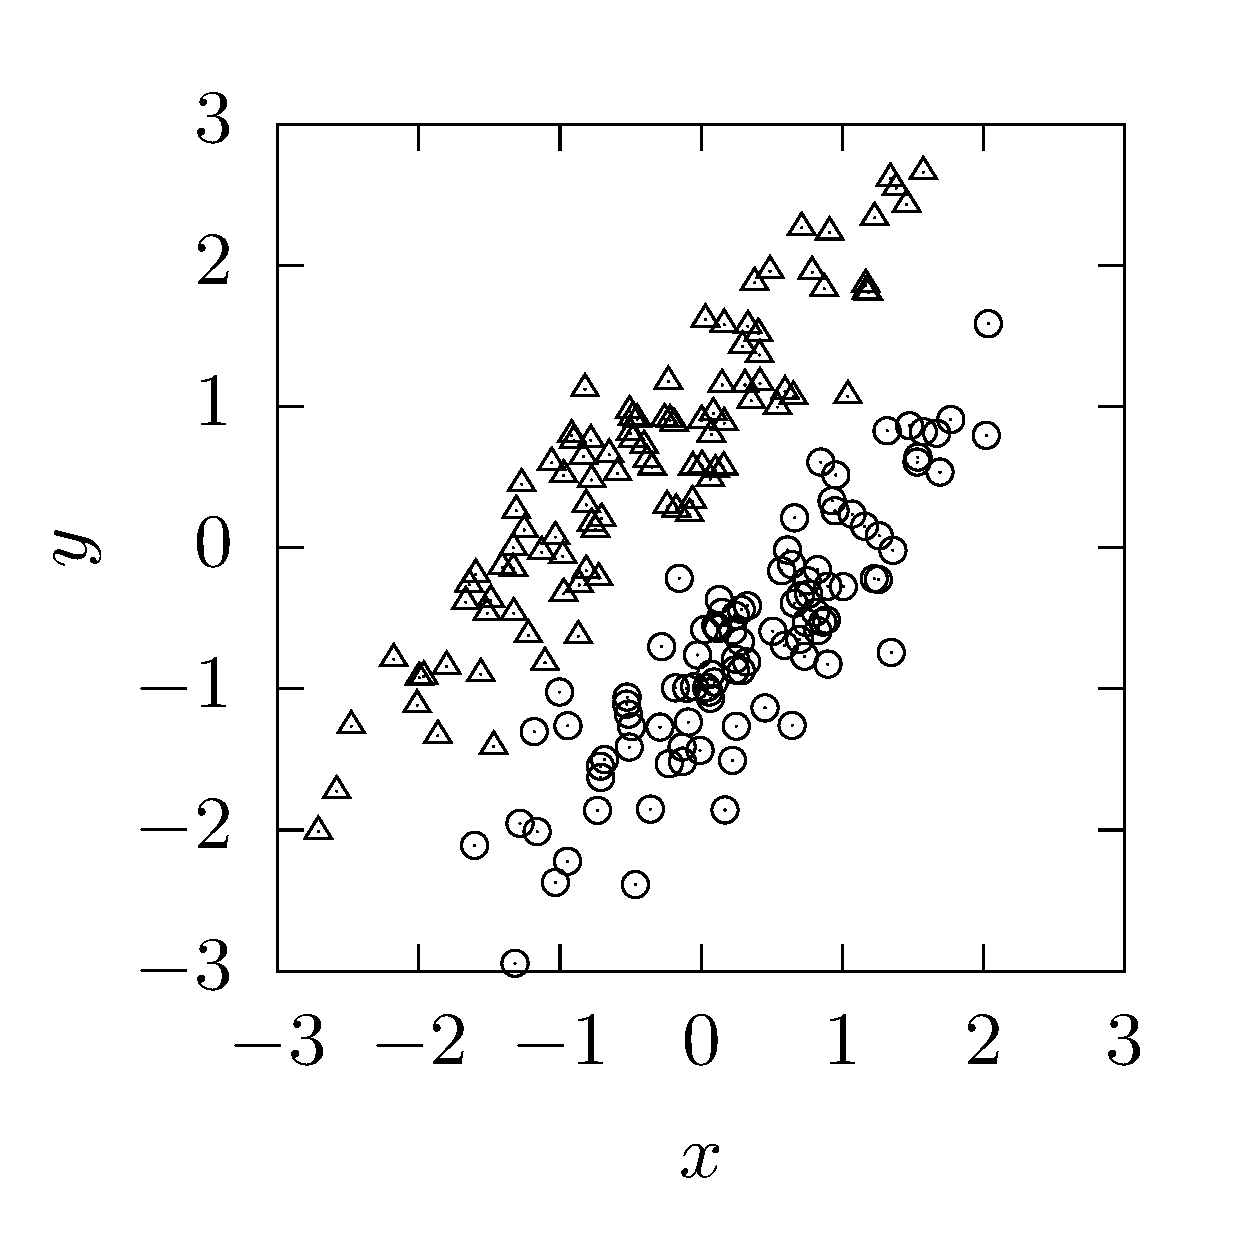
\includegraphics[scale=1.]{apdx_pca/corr_data.png}
    \end{subfigure}
    \begin{subfigure}{.49\textwidth}
        \centering
        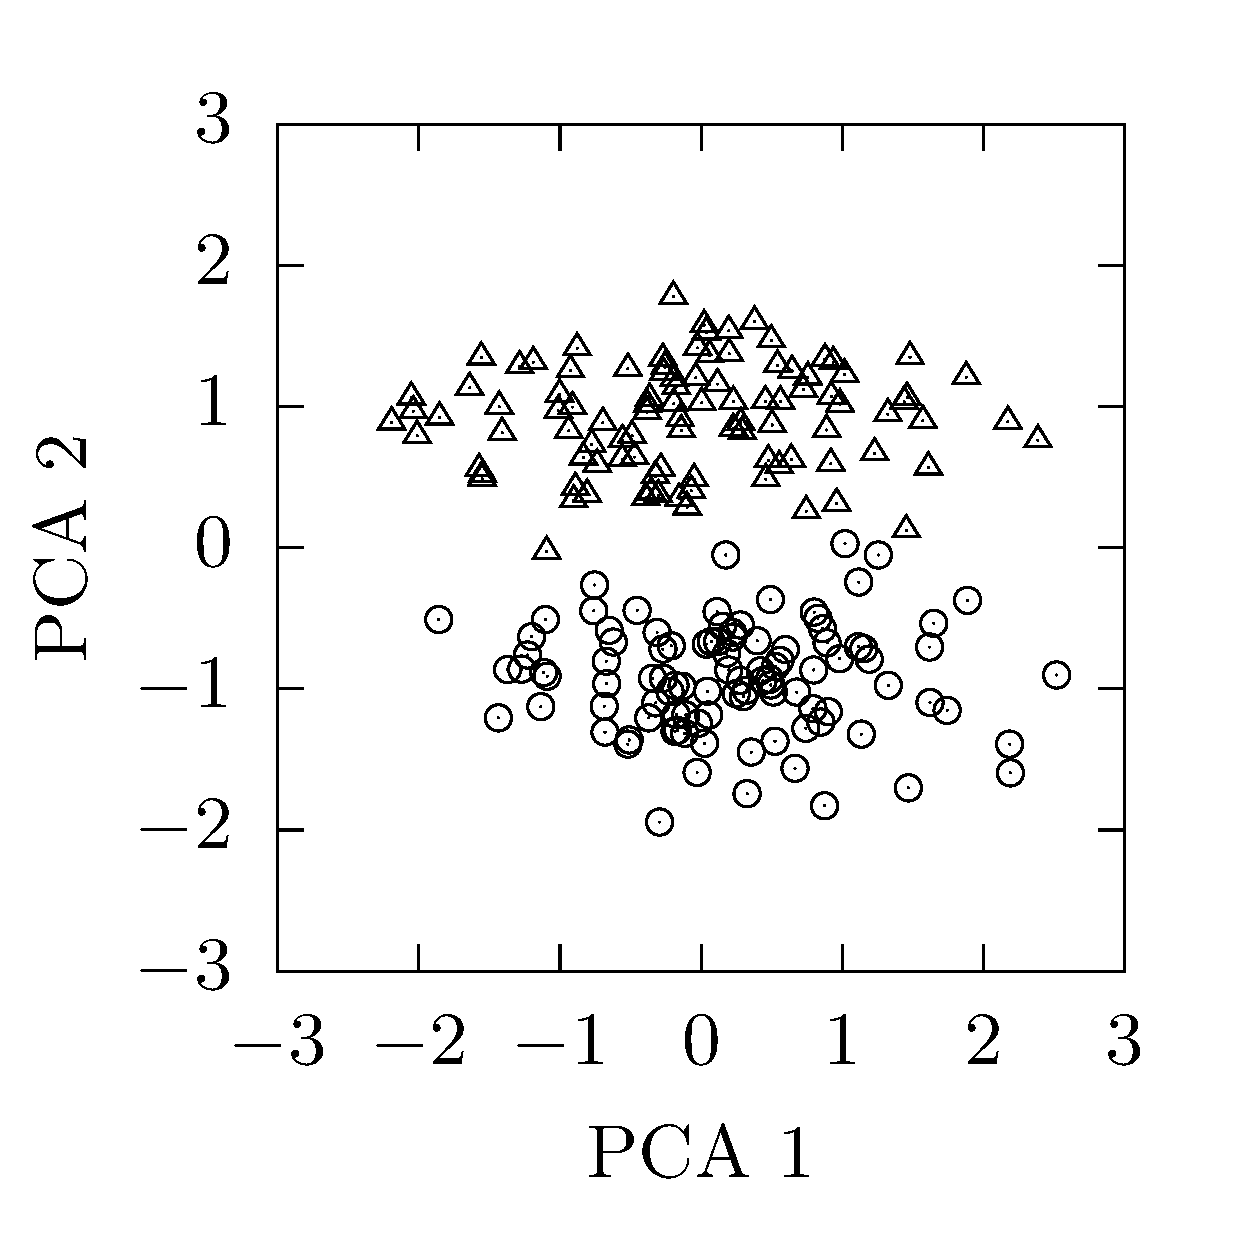
\includegraphics[scale=1.]{apdx_pca/corr_pca.png}
    \end{subfigure}
    \caption{Distribution of the two features $x$, $y$ of a joint data sample of two categories (circle and triangle). The canonical \gls{pca} transformation decorrelates the distribution by introducing rotated features PCA 1 and PCA 2, ordered by their respective standard deviations.}
    \label{fig:apdx_pca}
\end{figure}

In the given example, PCA 1 clearly is not helpful at all for distinguishing between the two categories, whereas PCA 2, albeit having a lower standard deviation, separates both distributions significantly.
We propose to use the $l_1$ Wasserstein distance for ordering the \gls{pca} components instead of the standard deviation.
As opposed to the more general $p$-th Wasserstein distance, the calculation of the $l_1$ distance is computational feasible, \ie{},
\begin{equation*}
    l_1(u, v) = \int \! \mathrm{d}x \, |U(x) - V(x)| \,,
\end{equation*}
where $U$ and $V$ are the cumulative distributions of $u$ and $v$, respectively (\cf{}~Ref.~\cite{wassersteinl1equiv}).
In Fig.~\ref{fig:apdx_hpca} we show the $l_1$ distance for our pseudo-experiment.
The $l_1$ distance appear to be a much better criterion for sorting \gls{pca} components than the standard deviation in the canonical approach.
We note that in direct comparison with other metrics, such as the Kolmogorov-Smirnov test, the Wasserstein $l_1$ distance is also much more stable (numerically) for distributions that differ strongly.
\begin{figure}[htbp]
    \centering
    \begin{subfigure}{.49\textwidth}
        \centering
        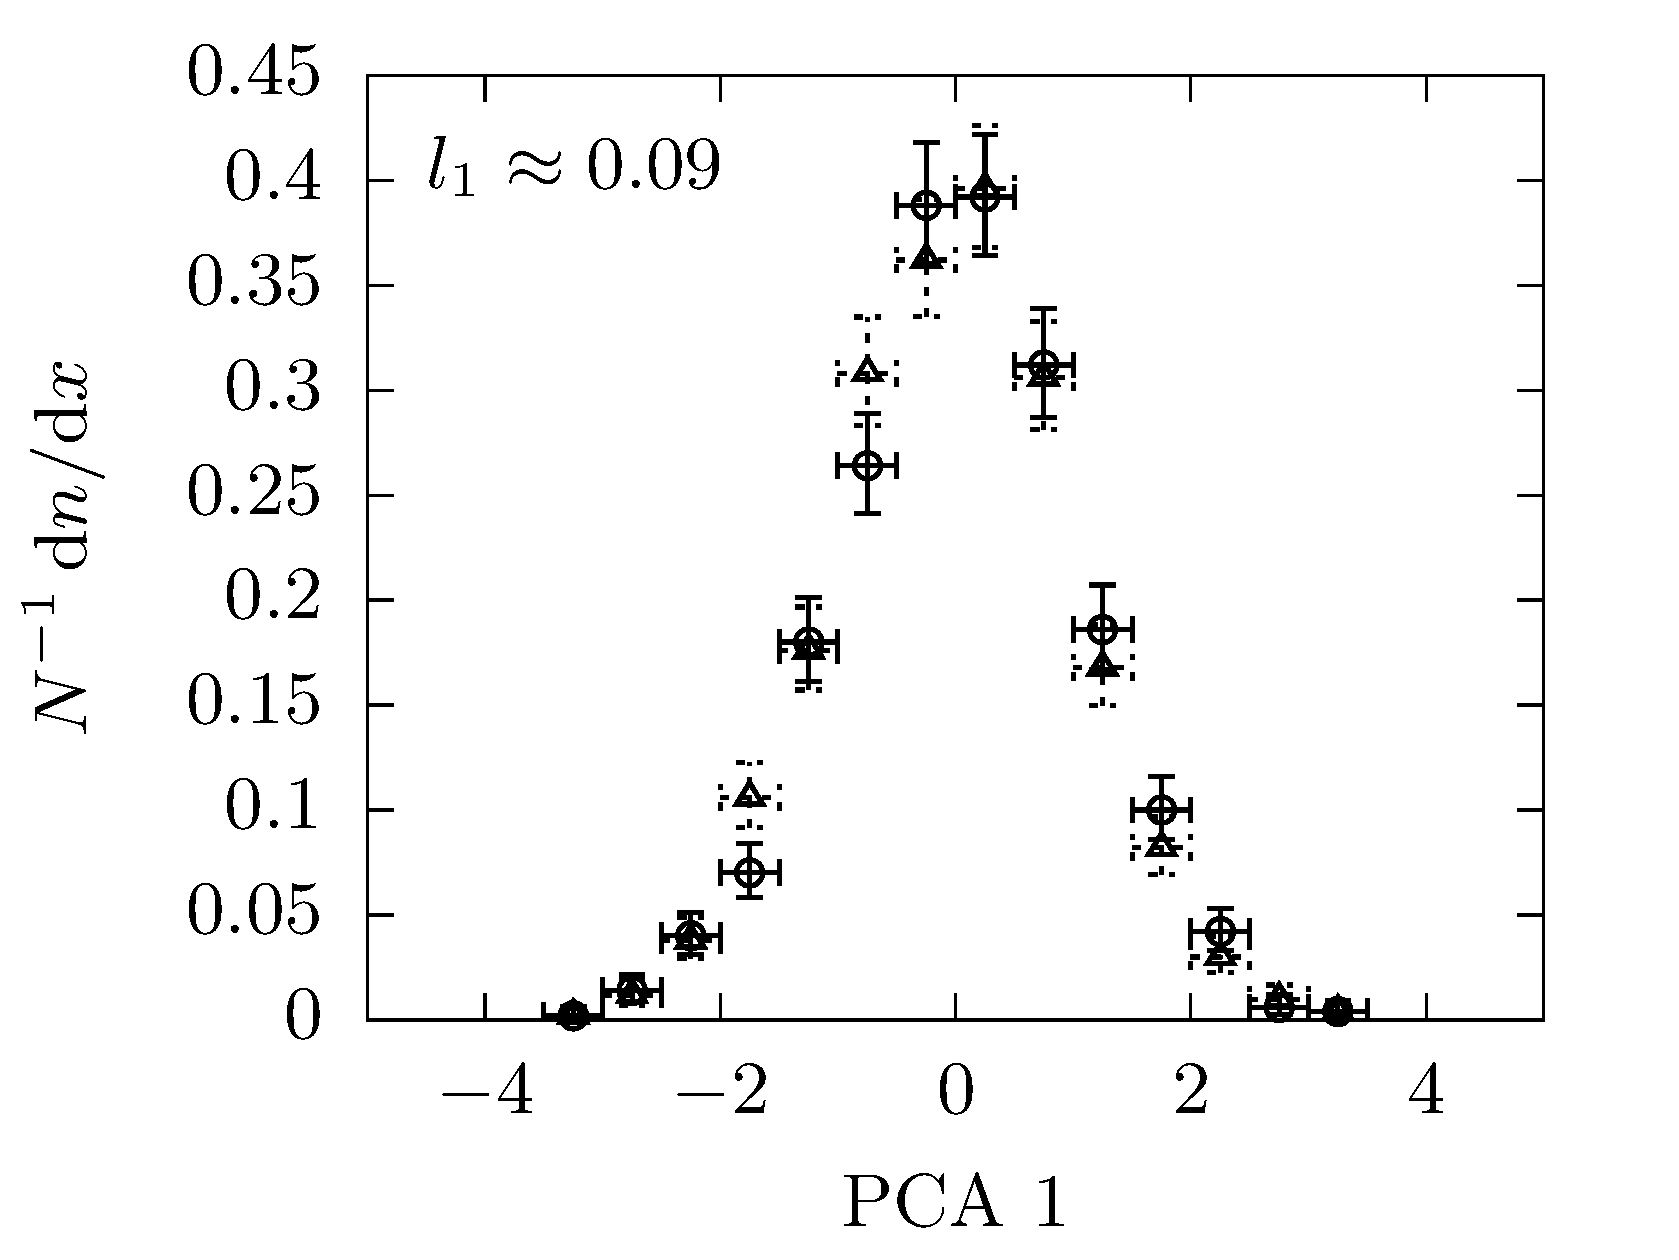
\includegraphics[scale=1.]{apdx_pca/hist_pca1.png}
    \end{subfigure}
    \begin{subfigure}{.49\textwidth}
        \centering
        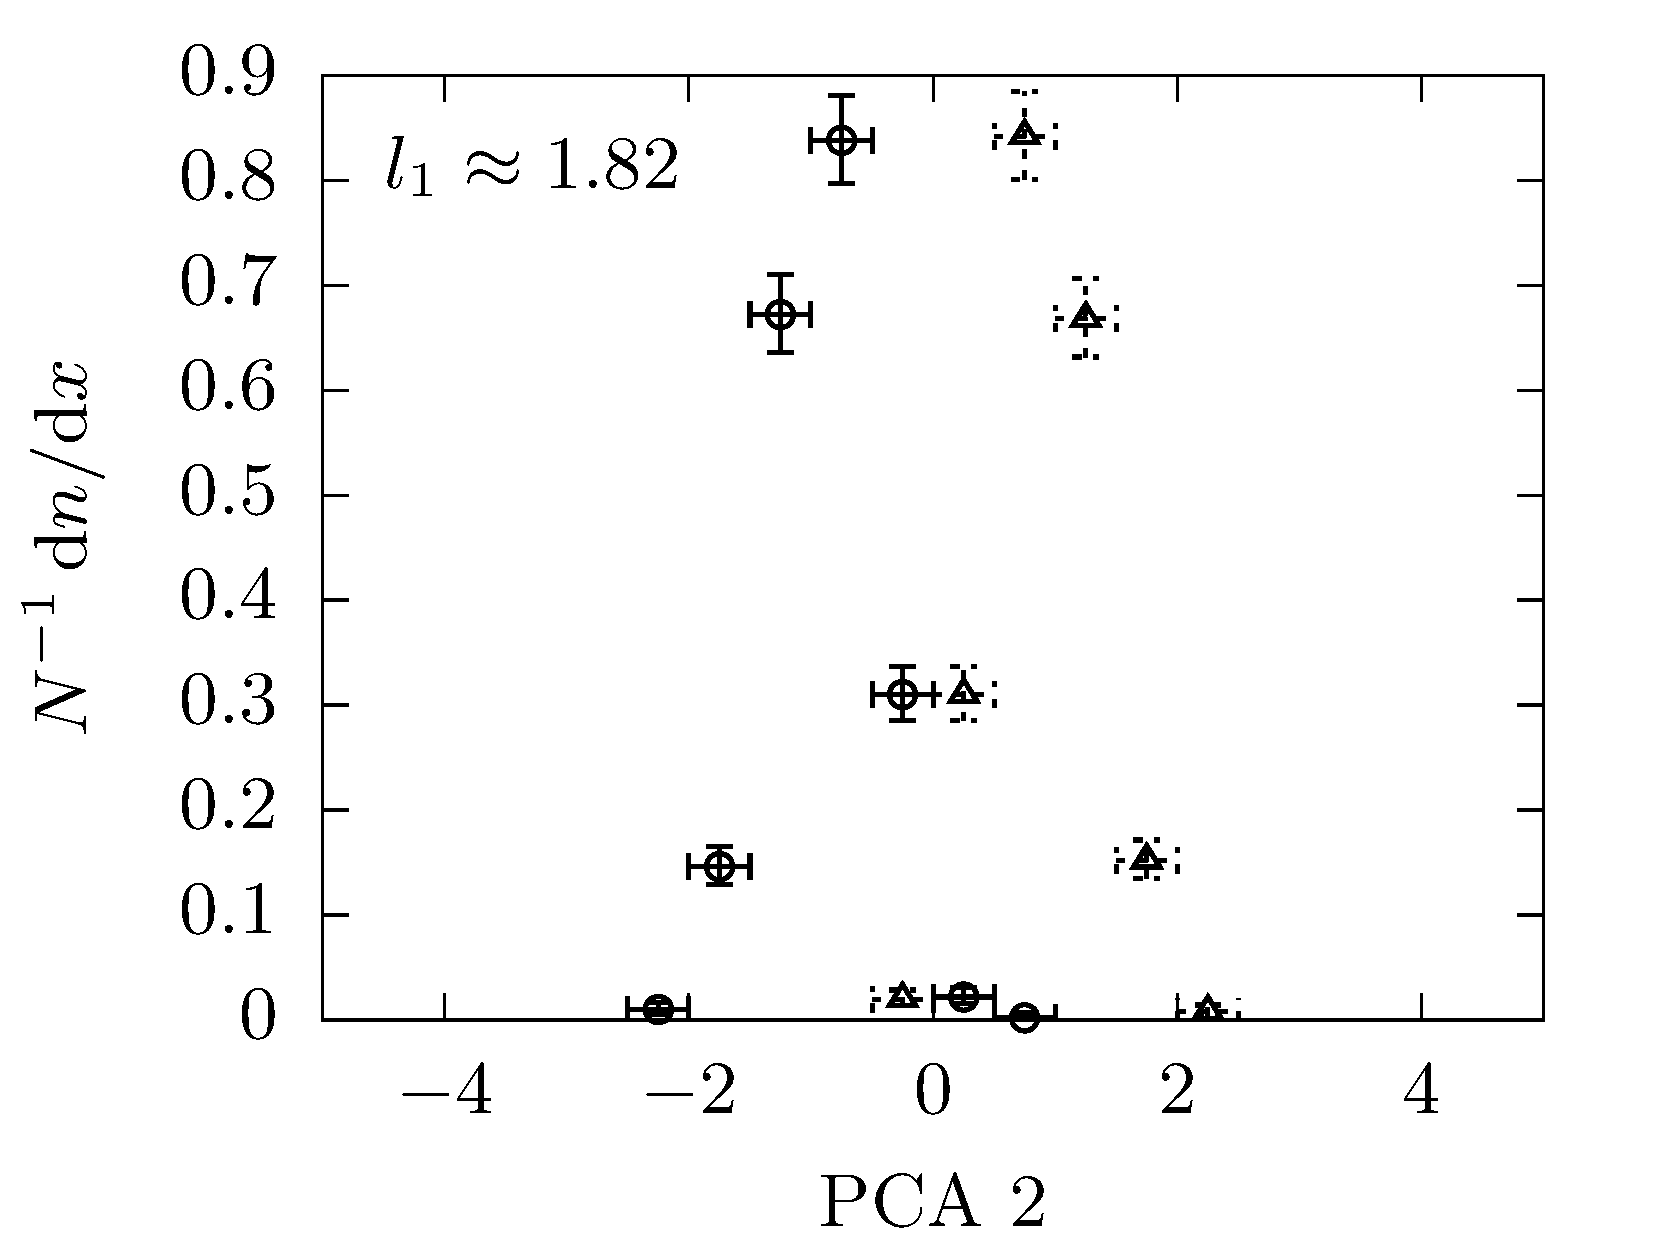
\includegraphics[scale=1.]{apdx_pca/hist_pca2.png}
    \end{subfigure}
    \caption{Distribution of PCA 1 (left) and PCA 2 (right). Even though PCA 1 has a larger standard deviation, it is not helpful at all for distinguishing between the two categories (circle and triangle). In our proposed solution the Wasserstein metric $l_1$ is used which rank PCA 2 well above PCA 1 in this case.}
    \label{fig:apdx_hpca}
\end{figure}
